\documentclass{beamer}

\input{../../spec_files/course_preamble.tex}
\subtitle{Foundations of Neuro-Symbolic AI}
\date{Summer Term 2026}
\author[FONS]{Alex Goessmann}
\institute[]{
    University of Applied Science Würzburg-Schweinfurt
%    Weierstrass Institute for Applied Analysis and Stochastic
}

%\newcommand{\techwstitle}{
%\small
%%Workshop \\
%Logik für Erklärbare KI:
%Technische Einführung in das ENEXA Projekt}
%\newcommand{\smalltechwstitle}{ENEXA Workshop}

%\newcommand{\techwsdate}{15.+16. July, 2024}

%\newcommand{\techwsauthors}{
%Alex Goessmann
%}

%\newcommand{\techwsinclude}{
%	\usepackage{../../spec/beamercolorthemeclaw}
%	\usepackage{/Users/alexgoessmann/Documents/ENEXA/latex_macros/beamer_template/beamerfontthemeclaw}
%	\usepackage{/Users/alexgoessmann/Documents/ENEXA/latex_macros/beamer_template/beamerinnerthemeclaw}
%	\usepackage{/Users/alexgoessmann/Documents/ENEXA/latex_macros/beamer_template/beamerouterthemeclaw}
%
%	\input{/Users/alexgoessmann/Documents/ENEXA/latex_macros/packages.tex}
%	\input{/Users/alexgoessmann/Documents/ENEXA/latex_macros/macros.tex}
%	\input{/Users/alexgoessmann/Documents/ENEXA/latex_macros/macros_tc.tex}
%	\input{/Users/alexgoessmann/Documents/ENEXA/latex_macros/tikz_blocks.tex}
%
%	\subtitle{\techwstitle}
%	\date[\techwsdate]{\techwsdate}
%	\author[\smalltechwstitle]{\techwsauthors}
%	\institute[]{\eupic}
%}

\newcommand{\techwschapterone}{I-Tensors}
\newcommand{\techwschaptertwo}{II-Probabilities}
\newcommand{\techwschapterthree}{III-Logics}
\newcommand{\techwschapterfour}{IV-Applications}

\newcommand{\eupic}{
\begin{center}
	%\includegraphics[width=4cm]{/Users/alexgoessmann/Documents/ENEXA/latex_macros/images/fundedEU.png}
\end{center}
}

\newcommand{\enexadateveublock}{
\begin{center}\begin{tikzpicture}
  	%\node [anchor=center] at (0,0) {\includegraphics[width = 1.5cm]{/Users/alexgoessmann/Documents/ENEXA/latex_macros/images/DATEV.png}};
	%\node [anchor=center] at (2.5,0.5) {\includegraphics[width = 3.5cm]{/Users/alexgoessmann/Documents/ENEXA/latex_macros/images/enexa.png}};
	%\node [anchor=center] at (2.55,-0.5) {\includegraphics[width = 3cm]{/Users/alexgoessmann/Documents/ENEXA/latex_macros/images/fundedEU.png}};
\end{tikzpicture}\end{center}
}


%% OLD
\newcommand{\aselectionvariable}{L}
\newcommand{\vselectionvariable}{L}
\newcommand{\fselectionvariable}{L}
\newcommand{\cselectionvariable}{L}
\newcommand{\individualorder}{n}
\newcommand{\variableof}[1]{\indvariableof{#1}}
\newcommand{\sindex}{s}
\newcommand{\pindex}{p}
\newcommand{\oindex}{o}
\newcommand{\exquery}{q}
%\newcommand{\datapointof}[1]{x^{#1}}
\newcommand{\atomicqueryof}[1]{g_{#1}}
\newcommand{\facsystem}{\shortcatvariables}
\newcommand{\margprobof}[1]{\probat{#1}}
\newcommand{\mlnprobabilityof}[1]{\expdistof{#1}}
%\newcommand{\oldenexadateveublock}{
%	\begin{center}
%	\begin{minipage}{0.2\textwidth}
%		\begin{center}
%			\includegraphics[width = 2.5cm]{images/DATEV.png}
%		\end{center}
%	\end{minipage}
%	\begin{minipage}{0.55\textwidth}
%		\begin{center}
%			\includegraphics[width=5.5cm]{images/enexa.png} \\
%			\includegraphics[width=5.5cm]{images/fundedEU.png} \\
%		\end{center}
%	\end{minipage}
%	\end{center}
%}

\title[Propositional Logics]{
	\techwschapterthree \\
	{\huge Introduction into Propositional Logics}
}

\usepackage{algorithmic}

\begin{document}

{\frame[plain]{\titlepage}}


\begin{frame}{Example: Reasons for a wet street}

Let there be a system described by three binary variables (being \var{True} or \var{False}):
\begin{itemize}
	\item $\var{Wet}$: Observation, that the street is wet.
	\item \var{Rained}: It had rained.
 	\item \var{Sprinkler}: The sprinkler had been on.
\end{itemize}

\begin{block}{Example of Reasoning}
	When we know that the formulas
	\begin{itemize}
		\item $\var{Rained}\Rightarrow\var{Wet}$ : Whenever it had rained, the street is wet.
		\item $\var{Rained}$: It had rained.
	\end{itemize}
	hold (i.e. = \var{True}), then it follows that the street is wet (i.e. \var{Wet} = \var{True}).
\end{block}

\end{frame}


\begin{frame}{Necessary Notation for a Logic}

Logic is build upon 
\textbf{Syntax}
\begin{itemize}
	\item How to formulate logical formulas? 
	\item Example: The formula $\var{Rained}\Rightarrow\var{Wet}$ represents the implication, that the street is wet whenever it had rained.
	\item Propositional Logics: The variables (or atomic formulas) are combined with logical connectives $\{\lnot, \land, \lor, \Rightarrow, \Leftrightarrow\}$ to build generic formulas.
\end{itemize}
and \textbf{Semantics} 
\begin{itemize}
	\item What do these formulas describe? 
	\item Example: From the formula $\var{Rained} \land \left( \var{Rained}\Rightarrow\var{Wet}\right)$ the formula $\var{Wet}$ follows.
	\item Propositional Logics: Each formula describes possible worlds, which are called models of a formula. Comparing the models defines the \textbf{entailment relation}.
\end{itemize}


\end{frame}



\begin{frame}{Model-theoretic semantics: Matrices represent formulas with two variables}

We mark the models (the possible worlds) of a formula, and choose an order by
\begin{itemize}
	\item \var{Wet} is False on the first column and True on the second
	\item \var{Rained} is False on the first row and True on the second
\end{itemize}
Then the model-theoretic semantics of $\var{Rained}\Rightarrow\var{Wet}$ is represented by the matrix:
\begin{align}
	\left(\var{Rained}\Rightarrow\var{Wet}\right) = 
	\begin{bmatrix}
	1 & 1 \\
	0 & 1 
	\end{bmatrix}
\end{align}

\end{frame}


\begin{frame}{Entailment by comparing the position of ones}

We summarize
\begin{align}
	\left(\var{Rained}\Rightarrow\var{Wet}\right) = 
	\begin{bmatrix}
	1 & 1 \\
	0 & 1 
	\end{bmatrix}
	\quad \text{and} \quad 
	\var{Rained} = 
	\begin{bmatrix}
	1 & 0 \\
	1 & 0 
	\end{bmatrix}
\end{align}
into
\begin{align}
	\var{Rained} \land \left(\var{Rained}\Rightarrow\var{Wet}\right) = 
	\begin{bmatrix}
	1 & 0 \\
	0 & 0 
	\end{bmatrix} \, . 
\end{align}
Comparing with 
\begin{align}
	\var{Wet} = 
	\begin{bmatrix}
	1 & 1 \\
	0 & 0 
	\end{bmatrix} \, . 
\end{align}
we notice, that every model of $\var{Rained} \land \left(\var{Rained}\Rightarrow\var{Wet}\right)$ is a model of $\var{Wet}$. We say that \var{Wet} is \textbf{entailed} and denote
\begin{align}
\Big( \var{Rained} \land \left(\var{Rained}\Rightarrow\var{Wet}\right) \Big) \models \var{Wet} \, .
\end{align}


\end{frame}



\begin{frame}{Model-theoretic semantics: Tensors represent multiple variables}

\textbf{Tensors} are a way to order all possible worlds in a system with multiple variables:
\begin{itemize}
	\item Each variable is associated with an \textbf{axis}.
	\item For each assignment to a variable we find a \textbf{coordinate}
\end{itemize}

\medskip 

\textbf{Example of three variables:}\\
 We associate the variable \var{Sprinkler} with a third direction 
\begin{center}
\begin{tikzpicture}
	\node (A) at (-3,0) {$\left(\var{Rained}\Rightarrow\var{Wet}\right) \land \var{Sprinkler}= $};
	\node (A) at (0,0) {
		$\begin{bmatrix}
			0 & 0 \\
			0 & 0 
		\end{bmatrix}$
	}; 
	\node (A) at (1,0.3) {
		$\begin{bmatrix}
			1 & 1 \\
			0 & 1 
		\end{bmatrix}$
	}; 
\end{tikzpicture}

\end{center}

\end{frame}


\begin{frame}{The curse of dimensionality in propositional logics}

\begin{block}{Factored System}
	A factored system is a set of $\atomorder$ variables $\catvariableof{\atomenumerator}$ indexed by $\atomenumeratorin$ each having $2$ assignments, which interact with each other.
\end{block}

The total number of states of a factored system is
	\[ 2^\atomorder \, . \]

\begin{block}{Curse of dimensionality}
	When reasoning about a factored system with many variables (i.e. $\atomorder$ is large), the naive enumeration of all models to formulas is infeasible.
\end{block}

The curse of dimensionality can be mitigated by smart distributed representations of the model marking tensors.

\end{frame}




\begin{frame}{Decomposition into logical connectives}

\textbf{Strategy:}
 Store the semantics of formulas $\exformula_1, \exformula_2$ and $\exformula_1\exconnective\exformula_2$ at each decomposition of the formula.

\medskip 

\begin{block}{Distributed Representation}
	The semantics of complex formulas is then stored by a set of semantics of the used logical connectives $\exconnective\in\{\lnot, \land, \lor, \Rightarrow, \Leftrightarrow\}$.
\end{block}

\medskip 

	\begin{minipage}{0.65\textwidth}
		A \textbf{graphical notation} depicts generic tensors:
		\begin{itemize}
			\item Tensors are rectangular boxes
			\item Each axis of a tensor is drawn by a leg to the box
	\end{itemize}
	\end{minipage}	
	\begin{minipage}{0.25\textwidth}
		\centering
		\begin{tikzpicture}[scale=0.35,yscale=-1]
			\draw[->] (0,1)--(0,-1) node[midway,left] {\tiny ${\exformula_1}$}; 
			\draw[->] (3,1)--(3,-1) node[midway,right] {\tiny ${\exformula_2}$}; 
	
			\draw (-1,-1) rectangle (4, -3);
			\node[anchor=center] (text) at (1.5,-2) {\small $\bencodingof{\circ}$};

			\draw[->] (1.5,-3) --(1.5,-5) node[midway,right]{\tiny ${\exformula_1 \exconnective \exformula_2}$};
		\end{tikzpicture}
	\end{minipage}	

\end{frame}


\begin{frame}{Encoding Logics using Tensors}

	
	Boolean states are represented by one-hot encodings
		\[ \onehotmapof{\truesymbol} = \tbasis = \begin{bmatrix}
			0 \\ 1
		\end{bmatrix}
		\quad \text{and} \quad \onehotmapof{\falsesymbol} = \fbasis = \begin{bmatrix}
			1 \\ 0
		\end{bmatrix}\, . \]
	
	The truth tables of logical connectives $\exconnective\in\{\land,\lor,\Rightarrow\}$ are represented by tensors $\bencodingof{\exconnective}\in\rr^{2\times 2 \times 2}$ defined as
	
	\begin{minipage}{0.5\textwidth}
	\begin{align*}
		\bencodingof{\exconnective} = \sum_{\exformula_1,\exformula_2\in\{\truesymbol,\falsesymbol\}} \onehotmapof{\exformula_1} \otimes \onehotmapof{\exformula_2} \otimes \onehotmapof{\exformula_1\exconnective\exformula_2}
	\end{align*}
	\end{minipage}
	\begin{minipage}{0.45\textwidth}
		\centering
		\begin{tikzpicture}[scale=0.35,yscale=-1]
			\draw[->] (0,1)--(0,-1) node[midway,left] {\tiny ${\exformula_1}$}; 
			\draw[->] (3,1)--(3,-1) node[midway,right] {\tiny ${\exformula_2}$}; 
	
			\draw (-1,-1) rectangle (4, -3);
			\node[anchor=center] (text) at (1.5,-2) {\small $\bencodingof{\circ}$};

			\draw[->] (1.5,-3) --(1.5,-5) node[midway,right]{\tiny ${\exformula_1 \exconnective \exformula_2}$};
		\end{tikzpicture}
	\end{minipage}	
	\medskip 
	
	%We interpret them by conditional probability distributions being the factors of the BPN (useful property for contractions).
	
	\medskip
	
	\textbf{Example:} Tensor Core to logical disjunction $\lor$ has the coordinates
	\begin{align*}
			\bencodingof{\lor}_{1,:,:}
			 = \begin{bmatrix}
			0 & 1 \\
			1 & 1 
			\end{bmatrix}
			\quad \text{and} \quad \bencodingof{\lor}_{0,:,:}
			 = \begin{bmatrix}
			1 & 0 \\
			0 & 0 
			\end{bmatrix} \, . 
	\end{align*}
		%Exploiting the standard duality of Graphical Models and Tensor Networks of their factors


\end{frame}



\begin{frame}{Encoding of Generic Formulas}
	The semantics of a \emph{formula $\exformula$} is a map
		\[ \exformula : \atomstates \rightarrow \{0,1\} \, . \]
	Given a formula $\exformula$ we call a world index by $(\atomindices) \in \atomstates$ a \emph{model} of $\exformula$, if $\exformula(\atomindices)=1$. \\
	\medskip 
	formulas are encoded by tensors
	\begin{align*}
		\bencodingof{\exformula} = \sum_{\atomindices\in[2]} \left( \bigotimes_{\atomenumeratorin} \onehotmapof{\atomlegindexof{\atomenumerator}} \right) \otimes \onehotmapof{\exformula(\atomindices)} \,
	\end{align*}
	depicted as
\begin{center}
	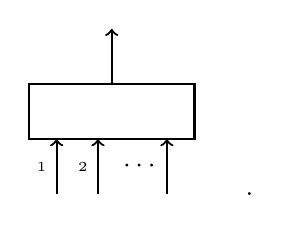
\begin{tikzpicture}[scale=0.35, thick] % , baseline = -3.5pt

\draw[->] (2,-1)--(2,1) node[midway,right] {\tiny ${\exformula}$};
\draw (-1,-1) rectangle (5,-3);
\node[anchor=center] (text) at (2,-2) {\small $\bencodingof{\exformula}$};
\draw[<-] (0,-3)--(0,-5) node[midway,left] {\tiny $\catvariableof{1}$};
\draw[<-] (1.5,-3)--(1.5,-5) node[midway,left] {\tiny $\catvariableof{2}$};
\node[anchor=center] (text) at (3,-4) {$\cdots$};
\draw[<-] (4,-3)--(4,-5) node[midway,right] {\tiny $\catvariableof{\atomorder}$};

\node[anchor=center] (text) at (7,-5) {$.$};

\end{tikzpicture}
\end{center}

\end{frame}



\begin{frame}{Tensor Calculus for Complex Formulas}

\begin{block}{Representation of Complex Formulas}
	The semantics of complex formulas are retrieved by \emph{contractions} of their connective semantics, which are summations of tensor coordinates among shared axes.
	\begin{itemize}
		\item Choose distributed representation to avoid contractions
		\item Only execute those contractions required by reasoning 
	\end{itemize}
\end{block}

Contractions can be depicted graphically by a \emph{Tensor Network}:
\begin{center}
	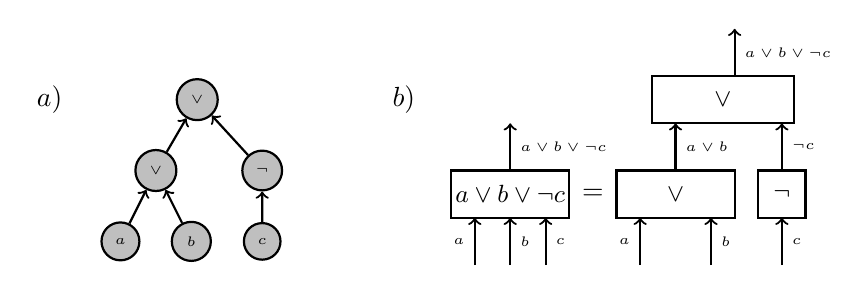
\begin{tikzpicture}[scale=0.3, yscale=-1, thick] % , baseline = -3.5pt

\begin{scope}[shift={(-15,0)}]

\node[anchor=center] (text) at (-3,-6) {${a)}$};

	\node [circle, draw, thick, fill=gray!50] (T1) at (0,0) {\tiny $a$};
	\node [circle, draw, thick, fill=gray!50] (T2) at (3,0) {\tiny $b$};
	\node [circle, draw, thick, fill=gray!50] (T3) at (6,0) {\tiny $c$};
	
	\node [circle, draw, thick, fill=gray!50] (and) at (1.5,-3) {\tiny $\lor$};
	\node [circle, draw, thick, fill=gray!50] (not) at (6,-3) {\tiny $\lnot$};	
	
	\draw [->] (T1) -- (and);
	\draw [->] (T2) -- (and);
	
	\draw [->] (T3) -- (not);	
	
	\node [circle, draw, thick, fill=gray!50] (head) at (3.25,-6) {\tiny $\lor$};
	
	\draw [->] (and) -- (head);
	\draw [->] (not) -- (head);			
\end{scope}

\node[anchor=center] (text) at (-3,-6) {${b)}$};

\draw[->] (0,1)--(0,-1) node[midway,left] {\tiny ${a}$}; 
\draw[->] (1.5,1)--(1.5,-1) node[midway,right] {\tiny ${b}$}; 
\draw[->] (3,1)--(3,-1) node[midway,right] {\tiny ${c}$}; 
\draw (-1,-1) rectangle (4, -3);
\node[anchor=center] (text) at (1.5,-2) {\small $\bencodingof{a \lor b \lor \lnot c}$};
\draw[->] (1.5,-3)--(1.5,-5) node[midway,right] {\tiny ${a \lor b \lor \lnot c}$}; 

\node[anchor=center] (text) at (5,-2) {${=}$};


\begin{scope}[shift={(7,0)}]

\draw[->] (0,1)--(0,-1) node[midway,left] {\tiny ${a}$}; 
\draw[->] (3,1)--(3,-1) node[midway,right] {\tiny ${b}$}; 
\draw[->] (6,1)--(6,-1) node[midway,right] {\tiny ${c}$}; 
	
\draw (-1,-1) rectangle (4, -3);
\node[anchor=center] (text) at (1.5,-2) {\small $\bencodingof{\lor}$};

\draw[->] (1.5,-3) --(1.5,-5) node[midway,right]{\tiny ${a \lor b}$};

\draw (5,-1) rectangle (7, -3);
\node[anchor=center] (text) at (6,-2) {\small $\bencodingof{\lnot}$};

\draw[->] (6,-3) --(6,-5) node[midway,right]{\tiny ${\lnot c}$};
	
\draw (0.5,-5) rectangle (6.5,-7);
\node[anchor=center] (text) at (3.5,-6) {\small $\bencodingof{\lor}$};
	
\draw[->] (4,-7) -- (4,-9) node[midway,right] {\tiny ${a \lor b \lor \lnot c}$};

%\draw (3,-9) rectangle (5,-11);
%\node[anchor=center] (text) at (4,-10) {$\truevectorat{}$};

\end{scope}

\end{tikzpicture}
\end{center}

\end{frame}


\begin{frame}{Logical Inference: Entailment}

The semantics of logics enable the calculation of logical consequences, framed logical inference.

\begin{definition}[Entailment]
	A propositional formula $\exformula$ is entailed by a formula $\kb$, if for each state $\atomindices$ with $\kb(\atomindices)=1$ we have $\exformula(\atomindices)=1$.
	We denote in this case
		\[ \kb \models \exformula \, . \]
\end{definition}

Approaches to automate the decision of entailment:
\begin{itemize}
	\item Proof-theoretic approaches: Inference rules such as Modus ponens
	\item Model-theoretic approaches: Check whether $\kb\land\lnot\exformula$ has a model.
\end{itemize}


\end{frame}



\begin{frame}{Deciding entailment by Contraction}

\begin{theorem}[Contraction Criterion for Entailment]
	We have $\kb\models\exformula$ (respectively $\kb\models\lnot\exformula$) if and only if 
		\[ \contractionof{\kb,\bencodingof{\exformula}}{\catvariableof{\exformula}} \parallel \onehotmapof{1} \quad \text{(respectively  } \contractionof{\kb,\bencodingof{\exformula}}{\catvariableof{\exformula}} \parallel \onehotmapof{0} \text{)} \, .\]
\end{theorem}

We depict this condition by
\begin{center}
	\begin{tikzpicture}[scale=0.35,thick] % , baseline = -3.5pt




\draw[->] (2,-1)--(2,1) node[midway,right] {\tiny $\catvariableof{\exformula}$};
\draw (-1,-1) rectangle (5,-3);
\node[anchor=center] (text) at (2,-2) {\small $\bencodingof{\exformula}$};
\draw[<-] (0,-3)--(0,-5) node[midway,left] {\tiny $\catvariableof{0}$}; 
\draw[<-] (1.5,-3)--(1.5,-5) node[midway,left] {\tiny $\catvariableof{1}$}; 
\node[anchor=center] (text) at (3,-4) {$\cdots$};
\draw[<-] (4,-3)--(4,-5) node[midway,right] {\tiny $\catvariableof{\atomorder\shortminus1}$}; 

\draw (-1,-5) rectangle (5,-7);
\node[anchor=center] (text) at (2,-6) {\small $\kb$};

%\node[anchor=center] (text) at (10,-4) {\small $\parallel$};
\draw (9,-3) -- (9,-5);
\draw (9.15,-3) -- (9.15,-5);

\draw[->] (13,-3)--(13,-1) node[midway,right] {\tiny $\catvariableof{\exformula}$};
\draw (12,-5) rectangle (14,-3);
\node[anchor=center] (text) at (13,-4) {\small $\onehotmapof{1}$};

\node[anchor=center] (text) at (16,-6) {$\cdot$};

\end{tikzpicture}
\end{center}

\end{frame}


\begin{frame}{Advantages of the Network Decomposition}

	\begin{block}{Model-theoretic Semantics by Tensor Networks}
		\begin{itemize}	
			\item \textbf{Tensors encode the models} of propositional formulas by their nonzero coordinates
			\item \textbf{Networks eliminate redundancies} when representing similar formulas
		\end{itemize}
		%Contractions with cores $\bencodingof{\exconnective}$ can be designed for various reasoning tasks.
	\end{block}

\medskip 

This is an implementation of the \textbf{neural paradigm}, resulting in
\begin{itemize}
	\item Effective representation: Latent variables by logical formulas
	\item Differential parametrization: Multilinearity with respect to each core tensor
\end{itemize}

\end{frame}


\begin{frame}{Implementations in \tnreason: \\
Subpackage \sprepresentation{}}

The subpackage \sprepresentation{} is dedicated to the implementation of logics.

\begin{center}
\begin{tikzpicture}[scale=0.27]

\draw[dashed] (-30,15) -- (12,15) -- (12,-3) -- (-30,-3) -- (-30,15);

\draw (-10,10) rectangle (10,14); 
\node [anchor=center] at (0,12) {\spapplication{}};

\node [anchor=center] at (-20,12) {\layerthreespec};
\draw[dashed] (-30,9) -- (12,9);
\node [anchor=center,blue] at (-20,6) {\layertwospec};

\draw[->] (6,10) -- (6,8);
\draw (2,4) rectangle (10,8); 
\node [anchor=center] at (6,6) {\spreasoning{}};
\draw[->] (6,4) -- (6,2);

\draw[->,blue] (-6,10) -- (-6,8);
\draw[blue] (-10,4) rectangle (-2,8); 
\node [anchor=center,blue] at (-6,6) {\sprepresentation{}};
\draw[->,blue] (-6,4) -- (-6,2);

\draw[dashed] (-30,3) -- (12,3);
\node [anchor=center] at (-20,0) {\layeronespec};

\draw (-10,-2) rectangle (10,2); 
\node [anchor=center] at (0,0) {\spengine};
\end{tikzpicture}
\end{center}

\end{frame}


\begin{frame}{Representation of Propositional Formulas}

Propositional formulas have three representations specified in the subpackage \sprepresentation{}:
\begin{itemize}
	\item \emph{Syntax} of formulas $\exformula$ is stored in a script language $\sencodingof{\exformula}$ based on nested lists of strings
	\item \emph{Semantics} of formulas is stored by tensor networks of connective cores
	\item Random variable representing the formula satisfaction
\end{itemize}

\end{frame}



\begin{frame}{Representation of Syntax}

In \tnreason, propositional syntax is represented by \emph{nested lists of strings}, for example:
		\begin{centeredscript}
			["and", ["not", "Rained"], ["imp", "Rained", "Wet"]]
		\end{centeredscript}
\medskip

Connective have a defined representation as strings:
\begin{center}
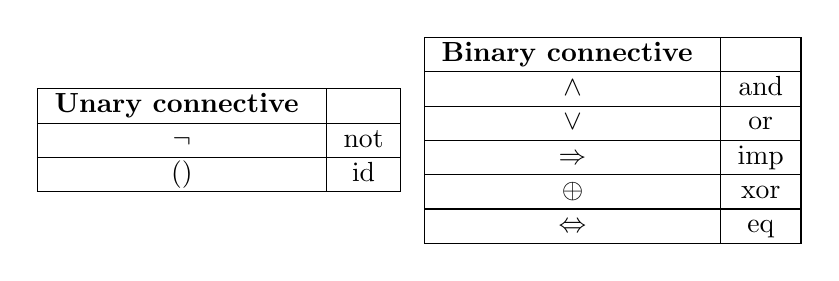
\begin{tikzpicture}
\node [anchor=center] at (0,0) {
	\begin{tabular}{|c|c|}
  	\hline
 	\textbf{Unary connective $\exconnective$} & \textbf{$\sencodingof{\exconnective}$} \\
  	\hline
 	$\lnot$ 	&  \stringof{not} \\
  	\hline
 	$()$		&  \stringof{id} \\
  	\hline
	\end{tabular}};
\node [anchor=center] at (5,0) {
	\begin{tabular}{|c|c|}
  	\hline
 	\textbf{Binary connective $\exconnective$} & \textbf{$\sencodingof{\exconnective}$} \\
  	\hline
 	$\land$ 		&  \stringof{and} \\
  	\hline
 	$\lor$ 		&  \stringof{or} \\
  	\hline
 	$\Rightarrow$ 	&  \stringof{imp} \\
  	\hline
	 $\oplus$ 		&  \stringof{xor} \\
  	\hline
	 $\Leftrightarrow$ &  \stringof{eq} \\
  	\hline
	\end{tabular}};
\end{tikzpicture}
\end{center}

Any other string is interpreted by an atomic formula (a so-called propositional symbol).

\end{frame}

\begin{frame}{Representation of Syntax}

Having strings representing
\begin{itemize}
	\item Connectives (by defined representations)
	\item Atomic Formulas (all other strings)
\end{itemize}
we represent formulas $\exformula_1\exconnective,\exformula_2$ 
\begin{centeredscript}
	[$\sencodingof{\exconnective}$, $\sencodingof{\exformula_1}$, $\sencodingof{\exformula_2}$]
\end{centeredscript}
where we apply the conventions
\begin{itemize}
	\item Connectives are at the 0th position in each list
	\item Further entries are either atoms as strings or encoded formulas itself
\end{itemize}
\end{frame}



\begin{frame}{Examples of representations}

%\begin{itemize}
%	\item 
	Atomic variable $\var{Rained}$ by
		\begin{centeredscript}
			$\sencodingof{\var{Rained}}$ = "Rained"
		\end{centeredscript}
%	\item 
	Negative literal $\lnot\var{Rained}$ by
		\begin{centeredscript}
			["not","Rained"]
		\end{centeredscript}
%	\item 
	Horn clause $\left(\var{Rained}\Rightarrow\var{Wet}\right)$ by 
 		\begin{centeredscript}
			["imp","Rained","Wet"]
		\end{centeredscript}
%	\item 
	Knowledge Base
	$(\lnot\var{Rained})\land(\var{Rained}\Rightarrow\var{Wet})$ by
		\begin{centeredscript}
			["and", ["not", "Rained"], ["imp", "Rained", "Wet"]]
		\end{centeredscript}
%\end{itemize}
		
\end{frame}


\begin{frame}{Semantics}

The recursive structure of the nested lists $\sencodingof{\exformula}$ is exploited in finding tensor network representations of $\exformula$.
The function
\begin{centeredscript}
	encoding.create\_raw\_cores()
\end{centeredscript}
creates the connective cores to $\sencodingof{\exformula}$ by 
\begin{itemize}
	\item When $\sencodingof{\exformula}$ a list, create $\bencodingof{\sencodingof{\exformula}[0]}$ and add to the tensor networks created by recursive calls to the subformulas $\sencodingof{\exformula}[1:]$
	\item Return empty list, when $\sencodingof{\exformula}$ is a string
\end{itemize}

Then we have
\begin{align*}
	\exformula = \contractionof{encoding.create\_raw\_cores(\sencodingof{\exformula}) \} \cup \{ \onehotmapof{1} }{\enumeratedatoms}
\end{align*}



\end{frame}


\end{document}













